\section{Definition of some variables}
Here the definition of some used variables are listed:
\begin{enumerate}
	\item $p_T$ balance : It is defined as 
			\begin{equation} \label{eq:ptBalance}
			A_{WV} = \frac{|p_T(V_h) + p_T(V_l)|}{p_T(V_h) + p_T(V_l)} 
			\end{equation}

	\item Boson centrality : It is defined as follows: 
			\begin{equation} \label{eq:bosonCentrality}
			\zeta_V = min\{\delta \eta_-, \delta \eta_+\} 
			\end{equation} 
			Where, \newline 
			$\delta \eta_- = min\{\eta(V_{had}), \eta(V_{lep})\}-min\{\eta_{j1},\eta_{j2}\}$ \newline 
			$\delta \eta_+ = max\{\eta_{j1},\eta_{j2}\}-max\{\eta(V_{had}), \eta(V_{lep})\}$

	\item Hadronic zeppenfeld : It is defined as 
		\begin{equation} \label{eq:HadZep}
		Zepenfeld\_WH = (\eta_{(AK8 jet)} - \frac{\eta_{j1} + \eta_{j2}}{2})/\delta \eta_{jj}
		\end{equation}

	\item Leptonic zeppenfeld : It is defined as 
		\begin{equation} \label{eq:LepZep}
		Zepenfeld\_WL = (\eta_{(Leptonic W)} - \frac{\eta_{j1} + \eta_{j2}}{2})/\delta \eta_{jj}
		\end{equation}

	\item Angular variables~\cite{AN:2012-463}: There are total five angular variables. They are $\cos\theta^{\ast}$, $\Phi_1$, $\Phi$, $\theta_1$, $\theta_2$ as shown in Fig. \ref{fig:anglesWWlvjj}. The angle $\cos\theta^{\ast}$ is the polar angle between the parton collision axis z and the $X$ decay axis $z'$, both defined in the $X$ rest frame. The angle $\Phi_1$ is the azimuthal angle between the
$zz'$ plane and the decay plane of hadronic $W$. The angles $\cos\theta^{\ast}$ and $\Phi_1$ are denoted as production angles because they depend on the production mechanism, $gg$ or $q\bar{q}$. The angle $\Phi$ is the angle between the decay planes of the two $W$ systems in the $X$ rest frame. The angle $\theta_i$ is the angle between the direction of the fermion f from $W \to f\bar{f}$ and the direction opposite the $X$ in the $W_i$ rest frame, where index i = 1, 2 refers to the first or second $W$ boson.  In the case of the $\cos\theta_i$ angle from the hadronic $W$, it is ambiguous as to which jet is originating from the fermion or
anti-fermion, so the angles is defined from $0$ to $\pi$ for the leading $p_T$ jet.  Finally, The angles $\Phi$, $\cos\theta_1$ and $\cos\theta_2$ do not depend on the production mechanism and are denoted as the helicity angles.
		
\end{enumerate}


%%%%%%%%%%%%%%%%%%%
\begin{figure}[ht]
  \centering
  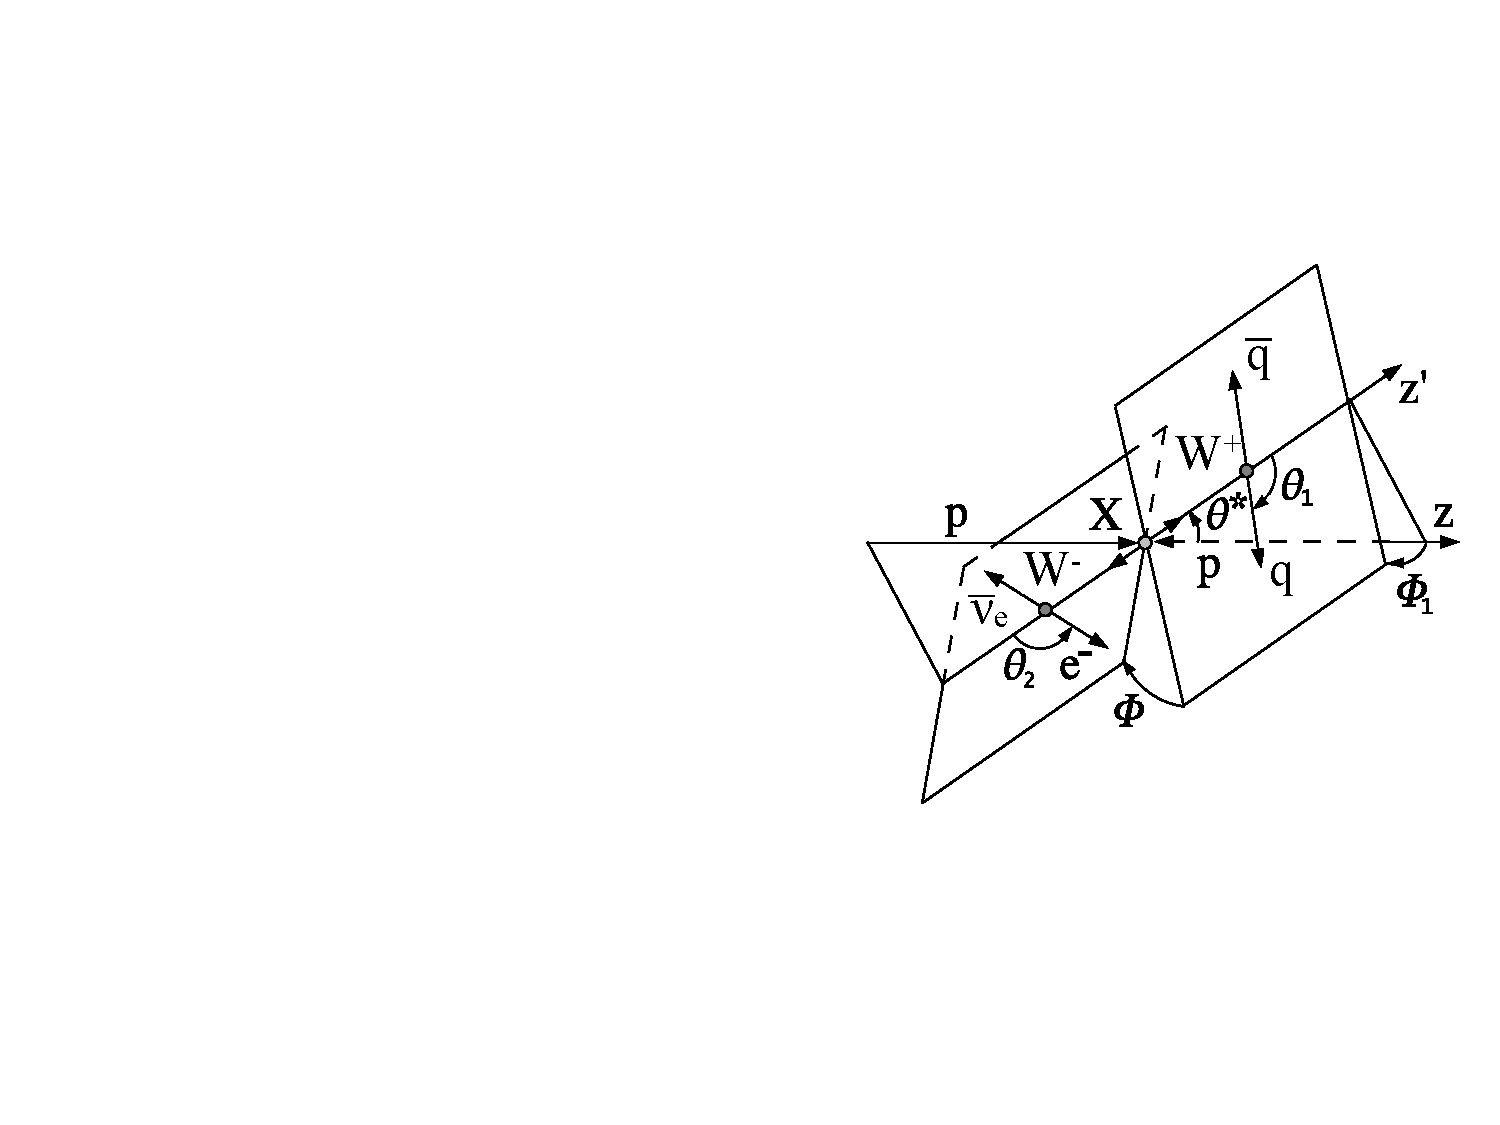
\includegraphics[width=0.5\textwidth]{Pictures/2012_MVAangles_wwlvjj.pdf}
  \caption{\label{fig:anglesWWlvjj}Angular definition for the $WW\to l\nu jj$ process}
\end{figure}
%%%%%%%%%%%%%%%%%%%

% \begin{table}[h!]
% \centering
% \caption{Definition of Variables}
% \label{Table:var1}
% \begin{tabular}{|p{0.6cm}|l|p{3.0cm}|p{9.0cm}|}
% \hline
% Sr. No. &	Symbol	&	Name			&	Definition	\\
% \hline
% \hline
% 1 & $A_{WV}$ 	& $p_{T}$ Balance	& .\newline $A_{WV} = \frac{|p_T(V_h) + p_T(V_l)|}{p_T(V_h) + p_T(V_l)}$ \newline\\
% \hline
% 2 & $\zeta_V$	& Boson Centrality	& $\zeta_V = min\{\delta \eta_-, \delta \eta_+\}$ \newline where, \newline $\delta \eta_- = min\{\eta(V_{had}), \eta(V_{lep})\}-min\{\eta_{j1},\eta_{j2}\}$ \newline $\delta \eta_+ = max\{\eta_{j1},\eta_{j2}\}-max\{\eta(V_{had}), \eta(V_{lep})\}$\newline\\
% \hline
% 3 & Zepenfeld\_WH &  Zeppenfeld w.r.t. hadronic W-boson & $(\eta_{(AK8 jet)} - \frac{\eta_{j1} + \eta_{j2}}{2})/\delta \eta_{jj}$\\
% \hline
% 4 & Zepenfeld\_WL &  Zeppenfeld w.r.t. leptonic W-boson & $(\eta_{(Leptonic W)} - \frac{\eta_{j1} + \eta_{j2}}{2})/\delta \eta_{jj}$\\
% \hline
% 1 &	$E_T^{miss}$	&	magnitude of missing transverse momenta vector &	It is defined as the projection on the plane perpendicular to the beams of the negative vector sum of the momenta of all reconstructed particles in an event.\\
% \hline
% 2 &	$M_T$		&	Transverse mass		&	$\sqrt{2p_T^lE_T^{miss}[1-cos(\Delta \phi (l,E_T^{miss})]}$\\
%   &			&				& 	where, $p_T^l$ is the transverse momentum of lepton	\\
%   &			&				&	$\Delta \phi (l, E_T^{miss})$ is the seperation in azimuthal angle between lepton and $E_T^{miss}$\\
% \hline
% \hline
% \end{tabular}
% \end{table}

% \begin{table}[t]
% \centering
% \caption{List of Variables}
% \label{my-label}
% \begin{tabular}{|l|l|}
% \hline
%  Description	& Definition	\\
% \hline
% $\eta$ separation between tag jets	&	$\Delta \eta_{jj}$	\\
% \hline
% tag jets invariant mass			&	$m_{jj}$		\\
% \hline
% $p_T$ of the leading VBF jet		&	$p_T^{J1}(VBF)$		\\
% \hline
% $p_T$ of the trailing VBF jet		&	$p_T^{J2}(VBF)$		\\
% \hline
% $p_T$ of the leading W-jet		&	$p_T^{J1}(W)$		\\
% \hline
% $p_T$ of the trailing W-jet		&	$p_T^{J2}(W)$		\\
% \hline
% hadronic asymmetry of VBF jets		&	$A_j (VBF)=\frac{p_T^{J1}-p_T^{J2}}{p_T^{J1}+p_T^{J2}}$ \\
% \hline
% hadronic asymmetry of W-jets		&	$A_j (Wjet)=\frac{p_T^{J1}-p_T^{J2}}{p_T^{J1}+p_T^{J2}}$ \\
% \hline
% $p_T$ of lepton				& 	$p_T(l)$		\\
% \hline
% missing energy value			&	$MET$			\\
% \hline
% \end{tabular}
% \end{table}




